\documentclass[11pt,a4paper,polish,thesis]{dcsbook}

\usepackage[T1]{fontenc}
\usepackage[utf8]{inputenc}
\usepackage{babel}
\usepackage{graphicx}

\setcounter{secnumdepth}{3}
\setcounter{tocdepth}{3}

\begin{document}

\author{Patryk Dąbrowski 100584\\ Aleksander Kędzierski 98875\\ Paweł Lampe 99277\\ Mateusz Sikora 99615}
\title{Platforma zarządzania zdarzeniami na urządzeniach mobilnych if\{y\}}
\supervisor{dr inż.~Jerzy Błaszczyński}
\date{Poznań, 2014}

\maketitle

\frontmatter

\tableofcontents{}

\mainmatter

\chapter{Wstęp}
%% Bardzo suchy wstęp zawierający to co ma być zawarte w klasycznym wstępie pracy inżynierskiej
\section{Opis problemu i koncepcja jego rozwiązania (motywacja?)}
Współczesne urządzenia mobilne dysponują ogromnym zbiorem możliwości. Nie są to już tylko telefony które dawniej służyły wyłącznie do komunikacji. Obecnie rynek pełen
jest urządzeń z zakresu; od tabletu do smartfonu. Mnogość typów urządzeń oraz tendencja do upodabniania się między sobą uniemożliwia jednoznaczne stwierdzenie do
czego właściwie służą.

Nie lepiej sytuacja ma się w przypadku programistów piszących aplikacje na urządzenia mobilne. Nie dość, że niemal każde urządzenie ma inny osprzęt, to co więcej, na
rynku figuruje kilka wiodących mobilnych systemów operacyjnych. Wszystko to wpływa dość drastycznie na charakter rynku aplikacji mobilnych. W większej części są to
proste aplikacje realizujące bardzo ściśle określone usługi. Prowadzi to do sytuacji, w której na przeciętnym smartfonie trzeba mieć 10-20 aplikacji które pozwolą osiągnąć stabilny poziom zadowolenia.

Gdyby istniała otwartoźródłowa aplikacja pozwalająca na stosunkowo prosty dostęp do możliwości telefonu oraz ułatwiająca proces programowania, wiele małych aplikacji
mogło by stać się prostymi receptami instruującymi aplikację--matkę jak wykonać stosunkowo proste zadania. W tym przypadku 10-20 małych aplikacji można by zamienić
na jedną zawierającą w środku 10-20 prostych kawałków kodu którymi można w pełni zarządzać.

Taka aplikacja oczywiście nie istnieje. Istnieją podobne, mniej lub bardziej udane rozwiązania. Wszystkie jednak są komercyjne co jest kluczową wadą. Zamkniętość kodu
-- bo o tym tutaj mowa, ogranicza zbiór osób zaangażowanych w tworzene i pielengnację kodu. Ma to ogromne implikacje na rozwój aplikacji, co z kolei uderza w jej
użytkowników. W przypadku jakiegokolwiek złożonego problemu, użytkownik nie jest w stanie samemu sprawdzić czy problem leży po stronie jego kodu, czy po
stronie kodu aplikacji.

Skoro wyżej wspomniana, otwartoźródłowa aplikacja nie istnieje, warto by ją stworzyć. Unicestwiło by to wszystkie wspomniane powyżej problemy. Taka też idea leży u
podstaw tej pracy. Stworzyć wolną, otwartoźródłową aplikację służącom przeciętnym użytkownikom. Co jednak nawet ważniejsze, stworzyć kod, który będzie mógł zostać
użyty przez zaawansowanych użytkowników-programistów.

\section{Cele i zakres pracy}
Postawowym celem niniejszej pracy, jest stworzenie otwartoźródłowej biblioteki uproszczającej dostęp do podzespołów urządzenia mobilnego. Jest to o tyle ważne, iż
tworzy warstwę abstrakcji nad systemem operacyjnym. Dzięki temu, kod który przykładowo przetwarza dane z GPS, pozostaje identyczny dla systemów Android, iOS tudzież
Windows Phone. Inna jest tylko implementacja biblioteki dla danej platformy. Niniejsza praca zakłada implementację biblioteki tylko dla systemu Android.

Drugim co do ważności celem, jest stworzenie przykładowej aplikacji prezentującej możliwości biblioteki. Z racji, iż implementacja biblioteki obejmuje tylko system
Android, implementacja aplikacji również. Fakt, iż aplikacja jest tylko przykładem, nie oznacza, że większość wykonanej pracy stanowi biblioteka. Wręcz przeciwnie.
Lwią część napisanego kodu stanowi aplikacja wraz z używanymi przez nią aplikacjami webowymi. Aplikacja bowiem, jako, że jest środowiskiem uruchomieniowym dla
krótkich kawałków kodu -- recept, potrzebuje zdalnego repozytorium bedącego niczym innym jak stroną internetową. Potrzebuje również serwera utrzymującego informacje
dla recept które korzystają z komunikacji w obrębie grup użytkowników. %TODO: dont share secret

Reasumując, kod który musi powstać, to biblioteka, aplikacja, repozytorium recept oraz serwer dla recept grupowych. %TODO: dont share secret
\section{Omówienie pracy}
Nixx nett hier
%% TODO
%% opis pracy jako dokumentu, kwestie treści etc.
%% streszczenia rozdziałów

\chapter{Wymagania}
%% wszelkie wymagania czyli:
%% wymagania funkcjonalne - to co wiemy
%% wymagania pozafuncjonalne - to czego na wstępie nie wiedzieliśmy np. 'recepty ma się łatwo pisać' - z tego w następnym rozdziale zrobi się problem który
%% został rozwiązany w postaci tych jarów
\section{Wymagania funkcjonalne}
\subsection{Przypadki użycia platformy}
\begin{description}
\item[UC1] Tworzenie Recepty
\item[1] Użytkownik wchodzi na stronę Targowiska.
\item[2]Użytkownik tworzy nową Receptę.
\item[3]Użytkownik pisze kod w edytorze online.
\item[3a]Użytkownik pisze kod lokalnie (np. w Eclipse) i przekazuje kod do Targowiska.
\item[4]Serwer kompiluje receptę.
\item[5]Użytkownik pobiera receptę na telefon.
\item[6]Recepta działa na telefonie.

\item[UC2] Ocena Recepty
\item[1] Użytkownik wchodzi na stronę Targowiska.
\item[2] Targowisko  


\end{description}
\subsection{Przypadki użycia Aplikacji - przykładowe Recepty}
\section{Wymagania pozafunkcjonalne}

\begin{tabular}{|p{2cm}|p{12cm}|}  \hline ID: &
PF01
\\ \hline Nazwa: &
System operacyjny dla aplikacji mobilnej	
\\ \hline Kategoria: &
Środowisko
\\ \hline Priorytet: &
Wysoki
\\ \hline Opis: &
Systemem operacyjnym aplikacji mobilnej jest Android w wersji minimum 2.1.

\\ \hline \end{tabular} \\\\\ \begin{tabular}{|p{2cm}|p{12cm}|}  \hline ID: &
PF02
\\ \hline Nazwa: &
Środowisko uruchomieniowe dla aplikacji serwerowej
\\ \hline Kategoria: &
Środowisko
\\ \hline Priorytet: &
Wysoki
\\ \hline Opis: &
Aplikacja serwerowa powinna działać na maszynie wirtualnej Java.

\\ \hline \end{tabular} \\\\\ \begin{tabular}{|p{2cm}|p{12cm}|}  \hline ID: &
PF03
\\ \hline Nazwa: &
Używane technologie
\\ \hline Kategoria: &
Technologie
\\ \hline Priorytet: &
Wysoki
\\ \hline Opis: &
Wykorzystane technologie nie mogą być płatne

\\ \hline \end{tabular} \\\\\ \begin{tabular}{|p{2cm}|p{12cm}|}  \hline ID: &
PF04
\\ \hline Nazwa: &
Zunifikowane środowisko programistyczne
\\ \hline Kategoria: &
Narzędzia
\\ \hline Priorytet: &
Wysoki
\\ \hline Opis: &
Programiści muszą zdecydować się na wspólne narzędzie do redagowania kodu (np. Eclipse)

\\ \hline \end{tabular} \\\\\ \begin{tabular}{|p{2cm}|p{12cm}|}  \hline ID: &
PF05
\\ \hline Nazwa: &
Ograniczone zużycie energii urządzenia mobilnego
\\ \hline Kategoria: &
Wydajność i niezawodność
\\ \hline Priorytet: &
Średni
\\ \hline Opis: &
Działanie aplikacji nie powinno w znaczącym stopniu skracać czasu pracy urządzenia na baterii

\\ \hline \end{tabular} \\\\\ \begin{tabular}{|p{2cm}|p{12cm}|}  \hline ID: &
PF06
\\ \hline Nazwa: &
Ograniczone zużycie zasobów urządzenia mobilnego.
\\ \hline Kategoria: &
Wydajność i niezawodność
\\ \hline Priorytet: &
Średni
\\ \hline Opis: &
Aplikacja nie powinna spowalniać działania innych aplikacji.

\\ \hline \end{tabular} \\\\\ \begin{tabular}{|p{2cm}|p{12cm}|}  \hline ID: &
PF07
\\ \hline Nazwa: &
Czas reakcji aplikacji na zdarzenie
\\ \hline Kategoria: &
Wydajność i niezawodność
\\ \hline Priorytet: &
Wysoki
\\ \hline Opis: &
Aplikacja powinna reagować na zdarzenia lokalne w mniej niż 2 sekundy

\\ \hline \end{tabular} \\\\\ \begin{tabular}{|p{2cm}|p{12cm}|}  \hline ID: &
PF08
\\ \hline Nazwa: &
Zgodność ze standardami kodowania dla języka Java
\\ \hline Kategoria: &
Zgodność ze standardami
\\ \hline Priorytet: &
Wysoki
\\ \hline Opis: &
Zarówno kod aplikacji mobilnej, jak i serwerowej powinien być redagowany zgodnie ze standardami dla języka Java

\\ \hline \end{tabular} \\\\\ \begin{tabular}{|p{2cm}|p{12cm}|}  \hline ID: &
PF09
\\ \hline Nazwa: &
Przechowywanie haseł
\\ \hline Kategoria: &
Bezpieczeństwo
\\ \hline Priorytet: &
Wysoki
\\ \hline Opis: &
Szyfrowane zapamiętywanie hasła użytkownika.

\\ \hline \end{tabular} \\\\\ \begin{tabular}{|p{2cm}|p{12cm}|}  \hline ID: &
PF10
\\ \hline Nazwa: &
Przechowywanie haseł
\\ \hline Kategoria: &
Bezpieczeństwo
\\ \hline Priorytet: &
Wysoki
\\ \hline Opis: &
Przechowywanie skrótu hasła na serwerze.
\\ \hline \end{tabular}

\chapter{Zarządzanie zdarzeniami na urządzeniach mobilnych}
%% wstęp vol. 2 - naświetlanie aktualnej wiedzy na temat tego co robimy, tutaj definiujemy pojęcia pokazujemy inne rozwiązania, ciśniemy po nich etc.
\section{Definicja pojęć}
\begin{itemize}
\item Podfunkcjonalność (ang. Feature) -- Część biblioteki zapewniająca Receptom dostęp do pozdbioru funkcjonalności Androida.
\item Zdarzenie (ang. Event) -- Zmiana stanu systemu, która powoduje uruchomienie kodu Recepty.
\item Recepta (ang. Recipe) -- Napisany przez użytkownika fragment kodu opisujący, co ma się zdarzyć po spełnieniu pewnych warunków.
\item Targowisko (ang. Market) -- Aplikacja internetowa pozwalająca tworzyć i pobierać Recepty.
\item Aplikacja -- Aplikacja androidowa wykorzystująca bibliotekę if\{Y\}. 
\item Serwer Grup -- Komputer z działającą aplikacją, która zarządza grupami użytkowników i Zdarzeniami Grupowymi.
\item Zdarzenie Grupowe -- Zdarzenie związane z Grupą, wysyłane lub odbierane przez Aplikację z Serwera Grup.
\item Grupa -- Zbiór użytkowników identyfikowalny przez nazwę zdefiniowany na Serwerze Grup.
\end{itemize}
\section{Istniejące rozwiązania}
\subsection{On X}
Aplikacja Microsoftu umożliwiającą kontrolowanie telefonu z Androidem używając kodu w JavaScripcie. Umożliwia wysyłanie Zasad (Rules) na telefon poprzez stronę internetową. Dostęp do funckcjonalości Androida jest zapewniony przez api w postaci Wyzwalaczy (Triggers) i Akcji (Actions). Cały system jest niestety połączony z Facebookiem i wymaga posiadania tam konta.
Na podstawie \cite{onx}.
\subsection{Tasker}

\chapter{Architektura platformy}
%% WYSOKI POZIOM ABSTRAKCJI ! Opis problemów, koncepcje rozwiązań, UMLe Diagramy Encji etc.
System składa się z biblioteki, przykładowej aplikacji appIFY oraz aplikacji działających na serwerze - Serwera Grup oraz Targowiska.
Aplikacja korzysta z biblioteki oraz komunikuje się z serwerem. Oprócz tego Serwer Grup oraz Targowisko udostępniają z poziomu przeglądarki takie funkcje jak rejestracja użytkowników czy tworzenie Recept. Kluczowym założeniem było maksymalne uproszeczenie kodu recept. 
TODO: Jeśli UI z weba nie będzie, to wyjebać wzmiankę

Kod Aplikacji jest podzielony na dwie części:
\begin{itemize}
\item bibliotekę IFY
\item aplikację appIFY
\end{itemize}
Celem takiego podziału jest ułatwienie tworzenia innych aplikacji opartych o bibliotekę.

\section{Recepty}
Miejscem, gdzie zawarta jest główna logika Aplikacji są Recepty -- są w nich opisane wszystkie zdarzenia, które mają nastąpić po spełnieniu pewnych ściśle określonych warunków. Docelowo będą one tworzone przez użytkowników i pobierane z Targowiska, jednak istnieją także przykładowe Recepty wbudowane w Aplikację, mające na celu ułatwienie użytkownikom tworzenia nowych na ich podstawie oraz rozszerzenie początkowej funkcjonalności aplikacji. 
Na receptę składają się:
\begin{itemize}
\item  opis używanych podfunkjonalności
\item  opis wymaganych parametrów
\item  opis jej właściwego działania
\end{itemize}
Deklarowanie używanych podfunkcjonalności ma dwa główne cele - po pierwsze, użytkownik widzi, czego używa recepta, co nieco poprawia jego bezpieczeństwo przy używaniu recept innych użytkowników, po drugie pozwala to inicjalizować nasłuchiwanie zdarzeń systemowych tylko wtedy, gdy istnieje aktywna recepta, która na nie reaguje - kod recepty nie musi inicjalizować większości podfunkcjonalności, wystarczy deklaracja ich używania. Wyjątkiem jest podfunkcjonalność grup, gdzie komunikację należy zainicjalizować.

Parametry pozwalają użytkownikowi na dostosowanie recepty do swoich wymagań, bez potrzeby pisania nowej. W naszych przykładowych receptach były to np. numer telefonu do wysłania SMS lub jego tekst czy też zasięg znajdowania znajomych na podstawie GPS.


TODO: Lanie wody poniżej?
Właściwa logika recepty jest zawarta w funkcji reakcji na zdarzenie. Wydaje się to sposób prostszy, niż na przykład ciągłe działanie recepty w osobnych wątku i odpytywanie Podfunkcjonalności o zdarzenia w kodzie recepty. Jest to rozwiązanie podobne do wzorca obserwatora, Recepta staje się jednak obserwatorem automatycznie na podstawie zadeklarowanych podfunkcjonalności, a wszytkie zdarzenia wywołują tą samą metodę w Recepcie. Takie rozwiązanie minimalizuje ilość kodu w recepcie, co było kluczowym celem.

\section{Biblioteka}
Biblioteka zawiera głównie API dostępne z poziomu recept, czyli między innymi Podfunkcjonalności, które agregują i upraszaczają dostęp do metod z API systemu Android. Oprócz tego znajduje się tam moduł odpowiedzialny za zarządzanie cycklem życia Recept i Podfunkcjonalności, który działa cały czas w tle. Podfunkcjonalności są inicjalizowane przez serwis przy uruchamianiu recepty, która deklaruje ich użycie. Zapewniają one dostęp do określonych funkcji, takich jak odczyt danych z sensorów, odbieranie i wysyłanie SMS'ów i wiele innych.
\section{Aplikacja kliencka}
Najważniejszym elementem Aplikacji jest interfejs użytkownika -- ekrany takie jak wyświetlanie listy dostępnych lub aktywnych recept, ustalanie ich parametrów i ich włączanie i wyłączanie. Dodatkowo aplikacja jest zintegrowana z Targowiskiem umożliwiając pobieranie z niego recept. Umożliwia też logowanie się do Serwera Grup.
TODO: Dop
\section{Targowisko}
1. geneza
2. rozwiązanie problemu
3. forkowanie
4. schmat bazy +
5. edytor online (artykuł?)
\begin{figure}[p]
  \centering
  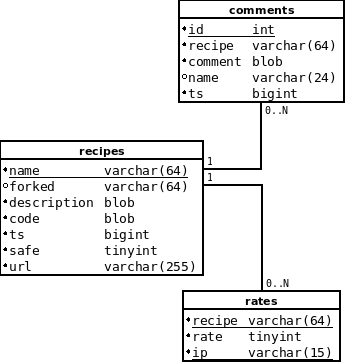
\includegraphics[scale=0.7]{./resources/market_db.png}
  %% \includegraphics[width=0.8\textwidth]{image.png}
  \caption{Schemat bazy danych targowiska}
  \label{fig:awesome_image}
\end{figure}
\section{Serwer}
% Jeśli nie chcesz mojej zguby serwer recept daj mi luby.

% TODO: zdanie do wyrzucenia? Sugerujemy, że serwer jest ważny, a potem gówno o nim piszemy.
% Jednym z trudniejszych i ważniejszych zadań do realizacji były recepty grupowe będące elementem odrózniającym projekt if{Y} od rozwiązań konkurencyjnych.

Głównym zadaniem przy tworzeniu recept grupowych jest przekazywanie wiadomości umożliwiajęce komunikację miedzy klientami i wymianę danych. 
Informacje niezbędne do działania tak ważnej funkcjionalności powinny być jednocześnie rozsyłane w prosty i łatwy do odczytania sposób przez każdą ze stron.

%tu opis innych rozwiązań które niewypaliły

Bezpośrednia komunikacja z użyciem połączenia internetowego między urządzeniami mobilnymi nie jest możliwa, dlatego niezbędnym było wprowadzenie urządzenia pośredniczącego w przesyłaniu danych. 
Serwer pełni w takim wypadku funkcję łacznika, dzieki czemu znany jest adres na jaki nalezy wysłac komunikat który ostatecznie ma dotrzeć do odbiorcy. 
Koncepcja ta opiera sie o tak zwany mechanizm odpytywania (ang. polling), który jest prosty do zaimplementowania ale jednocześnie spełnia wszytski wymagania stawiane w projekcie.
Odbieranie danych z serwera wykonywane poprzez cykliczne zapytania eliminuje problem łączności między aplikacja a pośredniczącym serwerem 

%tu jakiś diagram prdzedstawiajacy te koncepcję



\chapter{Opis implementacji}
%% NISKI POZIOM ABSTRAKCJI - detale techniczne - technologie, dokumnetacje, narzędzia, KOD, KOD, jeszcze trochę KODU, jakieś tricki w KODZIE etc.

\section{Recepty}
Recepty dziedziczą po klasie abstrakcyjnej YRecipe i implementują jej abstrakcyjne metody. Obrazuje to poniższy przykład recepty, która odrzuca wszystkie nadchodzące połączenia i wysyła SMS o zdefiniowanej przez użytkownika treści do dzwoniącej osoby.

\begin{verbatim}
public class YSampleCallsSMS extends YRecipe {
   @Override
   public void requestParams(YParamList params) {
      //Message to send in SMS
      params.add("MSG",YParamType.String, "Sorry, I'm busy.");
   }

   @Override
   public long requestFeatures() {
      return Y.Calls | Y.SMS;
   }

   @Override
   public void handleEvent(YEvent event) {
      //event is incoming call
      if(event.getId() == Y.Calls){
         YCallsEvent e = (YCallsEvent) event;
         //extract phone number
         String phone = e.getIncomingNumber();
         //discard call
         mFeatures.getCalls().discardCurrentCall();
         //send sms
         mFeatures.getSMS().sendSMS(phone, mParams.getString("MSG"));
      }
   }
   @Override
   public String getName() {
      return "YSampleCallsSMS";
   }
   @Override
   public YRecipe newInstance() {
      return new YSampleCallsSMS();
   }
}
\end{verbatim}
\subsection{Parametry -- requestParams}
Metoda requestParams ma za zadanie poinformować, jakich parametrów recepta wymaga do działania. Początkowo miała ona po prostu zwrócić listę i wyglądałaby tak:
\begin{verbatim}
public void requestParams() {
   YParamList params = new YParamList();
   params.add("MSG",YParamType.String, "Sorry, I'm busy.");
   return params;
}
\end{verbatim}
jednak tworzenie listy i zwracanie jej to dwie linie, które byłyby identyczne w każdej recepcie - ich wpisywanie może nieco irytować. Wobec tego obecnie metoda ta przyjmuje jako argument pustą listę parametrów, którą ma za zadanie wypełnić, zgodnie z założeniem maksymalnego uproszczenia kodu recepty.

\subsection{Używane Podfunkcjonalności -- requestFeatures}
Metoda requestFeatures ma za zadanie poinformować system, jakich Podfunkcjonalności używa Recepta. Początkowo była ona podobna do requestParams i wypełniała listę nowymi obiektami odpowiedniej klasy, co wyglądałoby tak:
\begin{verbatim}
public void requestFeatures(YFeatureList features) {
   features.add(new YCallsFeature());
   features.add(new YSMSFeature());
   return params;
}
\end{verbatim}
Przy takim rozwiązaniu jednak tworzyło się wiele niepotrzebnych obiektów - poprawnie zainicjalizowane Podfunkcjonalności powinny być tworzone w systemie tylko raz. Wystarczyłaby zatem lista identyfikatorów, pozwalająca zainicjalizować odpowiednie Podfunkcjonalności. Identyfikatorów jest jednak na tyle mało, że tak naprawdę nie potrzeba prawdziwej listy, wystarczy maska bitowa. Ułatwia to przesyłanie takiej listy między modułami systemu, działającymi w różnych procesach - nie trzeba się martwić o implementację w liście interfejsu Parcelable, potrzebnego do przesyłania obiektów między procesami w Androidzie.

Ostatecznie zatem metoda ta zwraca liczbę typu long, będącą sumą bitów reprezentujących poszczególne Podfunkcjonalności. Mapowanie tych bitów jest zawarte w klasie Y.
\begin{verbatim}
[...]
public static final long Wifi = 0x0008;
public static final long GPS = 0x00010;
[...]
\end{verbatim}
Dodatkowo warto zauważyć, że nazwy stałych w tej klasie odpowiadają nazwom Podfunkcjonalności oraz Zdarzeń - dla stałej {\bf ABC} klasa z Podfunkcjonalnością nazywa się Y{\bf ABC}Feature, a zdarzenie - Y{\bf ABC}Event. Powinno to ułatwić automatyczne generowanie kodu recept. 

\subsection{Logika recept -- handleEvent}
Metoda jest wywoływana, gdy w systemie nastąpi zdarzenie związane z Podfunkcjonalnością używaną przez receptę. W argumencie podawane jest zdarzenie -- obiekt typu YEvent. 
Aby poznać szczegóły zdarzenia recepta musi sprawdzić jego typ porównując wartość zwracaną przez getId() ze stałymi z klasy Y. Następnie można zrzutować zdarzenie na odpowiedni typ i poznać jego szczegóły. 

%Niestety nie udało się tutaj znaleźć bardziej eleganckiego rozwiązania. 
Recepty mogą też zażądać pewnych danych od systemu, które są dostarczane asynchronicznie - na przykład przetłumaczenie danych z GPS na adres (Geocoder). Wyniki tego typu operacji również są przekazywane do recepty jako typ YEvent.

Z poziomu obsługi zdarzenia można także dostać się do listy Podfunkcjonalności oraz listy Parametrów poprzez metody getFeatures() i getParams(). Początkowo dostęp do Podfunkcjonalności odbywał się następująco:
\begin{verbatim}
YCallsFeature cf = (YCallsFeature) mFeatures.get(Y.Calls);
\end{verbatim}
Jednak wymuszało to rzutowanie i niepotrzebnie wydłużało kod, zatem obecnie klasa YFeatureList zawiara metody pobierające konkretne podfuncjonalności.
\begin{verbatim}
public YCallsFeature getCalls() {
    return (YCallsFeature) get(Y.Calls);
}
\end{verbatim}
Ich utrzymanie może być później nieco kłopotliwe - każde dodanie Podfunkcjonalności będzie wymagało dodania odpowiedniej metody, jednak uproszczenie kodu recepty jest tego warte.

Warto również wspomnieć, że metoda handleEvent może rzucić dowolny wyjątek - recepta zostanie wówczas wyłączona. Ułatwia to pisanie recept zapewniając jednocześnie stabilność aplikacji.

\subsection{Aktywacja}
Fragmenty kodu przedstawione poniżej różnią się od oryginalnych -- dla poprawy czytelności nie ma w nich tworzenia logów.
Recepta jest aktywowana przez serwis, na podstawie nazwy i listy parametrów.
\begin{verbatim}
   public int enableRecipe(String name, YParamList params) {
      int id = ++mRecipeID;
      int timestamp = (int) (System.currentTimeMillis() / 1000);
      YRecipe recipe = mAvailableRecipesManager.getRecipe(name).newInstance();
      long feats = recipe.requestFeatures();
      YFeatureList features = new YFeatureList(feats);
      initFeatures(features);
      params.setFeatures(feats);
      if(!recipe.initialize(this, params, features, id, timestamp)){
         return 0;
      }
      for (Entry<Long, YFeature> entry : features) {
         entry.getValue().registerRecipe(recipe);
      }
      mActiveRecipesManager.put(id, recipe);
      return id;
   }
\end{verbatim}
Generowany jest ID konretnej instancji recepty oraz zapisywany jest czas jej uruchomienia.
Następnie tworzony jest nowy obiekt typu właściwego do konkretnej recepty. W tym celu znajdujemy niezainicjaliwaną receptę w bazie i posługujemy się metodą newInstance - nie w tym miejscu kodu nie jest znana nazwa klasy recepty, aby móc wprost wywołać konstruktor. Innym możliwym rozwiązaniem byłby mechanizm refleksji, jednak to rozwiązanie jest szybsze, gdyż nie mogą być optymalizowane przez maszynę wirtualną \cite{java}
Dalej na podstawie zwróconej przez receptę maski bitowej tworzona jest lista podfunkcjonalności wymaganych przez receptę do działania. Następnie podfunkcjolności które już są aktywne są wpisywane do listy w miejsce niezainicjalizowanych, a pozostałę są aktywowane i dodawane do listy aktywnych.

\begin{verbatim}
   protected void initFeatures(YFeatureList features) {
      for (Entry<Long, YFeature> entry : features) {
         Long featId = entry.getKey();
         YFeature feat = mActiveFeatures.get(featId);
         if (feat != null) {
            entry.setValue(feat);
         } else {
            feat = entry.getValue();
            feat.initialize(this);
            mActiveFeatures.add(feat);
         }
      }
   }
\end{verbatim}
Po zainicjalizowaniu Podfunkcjonalności Recepta jest w nich rejestrowana. Umożliwia to wywoływanie metody handleEvent w odpowiedzi na zdarzenia systemowe. 
% TODO: bibliografia do leniwego
Warto zauważyć, że zarówno Recepty jak i Podfunkcjonalności są leniwie inicjalizowane, co pozwala tymczasowo używać niezainicjalizowanych obiektów, a potem zastępować je innymi bez wykonywania zbędnych operacji. 

\begin{verbatim}
   public final boolean initialize(IYRecipeHost host, YParamList params,
         YFeatureList features, int id, int timestamp) {
      mHost = host;
      mParams = params;
      mFeatures = features;
      mId = id;
      mTimestamp = timestamp;
      Log = new YLogger(createTag(mId, getName()), host);
      try {
         init();
      } catch (Exception e) {
         e.printStackTrace();
         return false;
      }
      return true;
   }
\end{verbatim}

Sama inicjalizacja recepty to głównie wstrzyknięcie jej parametrów, Podfunkcjonalności, ID oraz czasu aktywacji. Oprócz tego jest tworzony Dziennik Recepty oraz jest wywoływana funkcja init() zawierająca kod inicjalizacyjny specyficzny dla danej recepty (na przykład otwarcie kanału komunikacji z Serwerem Grup). Takie rozwiązanie w połaczeniu w modyfikatorem final w metodzie zapewnia jej wywołanie, a kod recepty nie ma dostępu do danych, które nie są mu potrzebne. Dodatkowo funkcja init() może się nie powieść - wyjątki są wówczas łapane, metoda initialize() zwraca wówczas wartość false, a recepta nie jej dodawana do listy aktywnych.
%TODO Dziennik -> słowniczek



\section{Biblioteka}
\subsection{Serwis}
Wszystkie operacje odbywające się w bibliotece działają w kontekście serwisu, zaimplementowane w klasie YAbstractRecipeService.
Serwis w Androidzie to komponent aplikacji przeznaczony do długotrwałego wykonywania operacji w tle, nieposiadający interfejsu użytkownika. \cite{android.serwis}
Wszelka komunikacja z użytkownikiem przebiega poprzez aplikację, która komunikuje się z serwisem.

\section{Aplikacja kliencka}
\subsection{Moduły dostępu do systemu}
\subsection {Obsługa Targowiska}
Moduł obsługi Targowiska jest odpowiedzialny za  wyświetlanie danych dotyczących recept dodanych w aplikacji internetowej oraz pobieranie plików .jar ze skompilowanymi receptami, które następnie są zapisywane na pamięci wewnętrznej urządzenia mobilnego (w celu zachowania tej samej bazy recept w przypadku w którym użytkownik usunie zewnętrzny nośnik pamięci z urządzenia). Informacje o plikach z receptami (ich nazwy oraz ścieżki) przechowywanymi na telefonie zapisywane są po pomyślnym pobraniu w  bazie danych.
\subsection {Obsługa pobranych  Recept}
W aplikacji klienckiej zrealizowanej w ramach pracy inżynierskiej rozróżniamy dwa typy recept - wbudowane i pobrane z Targowiska. Kod źródłowy recept pierwszego typu jest zawarty w kodzie źródłowym Aplikacji. W przypadku recept pobranych z Targowiska, w celu umożliwienia Aplikacji korzystania z takiej recepty wykorzystywane jest archiwum .jar, zawierające plik .dex (Dalvik Executable) z kodem wykonywalnym  zrozumiałym dla maszyny wirtualnej Dalvik. Informacje potrzebne to załadowania kodu recepty (nazwa klasy oraz ścieżka dostępu do pliku .jar) przechowywane są w bazie danych recept pobranych na urządzenie. 
\subsection{Komunikacja serwisu z aplikacją kliencką}
W opisie komunikacji między aplikacją kliencką a serwisem recept wykorzystane będą klasy z Android SDK - Messenger, Bundle i interfejs Parcelable. Klasa Messsenger umożliwia przesyłanie danych między procesami. \cite{android.mesage} Do opakowania danych wykorzystywana jest klasa Bundle, która przechowuje obiekty i typy prymitywne w postaci mapy. Warto wspomnieć, że aby uzyskać możliwość przechowania obiektu w tej klasie, musi on implementować interfejs Serializable lub Parcelable. Pierwszy z nich umożliwia serializacje obiektów znaną z Javy, natomiast drugi został zaimplementowany w Android SDK w celu zwiększenia wydajności serializacji. W pracy inżynierskiej wykorzystujemy drugi z mechanizmów. Po uruchomieniu serwis recept wystawia obiekt implementujący interfejs IBinder służący do wiązania obiektów klasy Activity z obiektami klasy Service,  z którym z kolei jest związany obiekt klasy Messenger zaimplementowany w serwisie recept. Aby ustanowić połączenie, Aktywność musi stworzyć obiekt klasy Intent, sparametryzować go klasą Service z którą nawiązywane jest połączenie i zapewnić obiekt implementujący interfejs ServiceConnection, który reaguje na uzyskanie i zerwanie połączenia, a następnie wywołać metodę bindService jako parametr podając wspomniany wyżej obiekt klasy Intent. Po nawiązaniu połączenia następuje wymiana obiektów klasy Messenger, dzięki czemu możliwa jest komunikacja w obie strony. Warto dodać, że ten mechanizm komunikacji jest asynchroniczny. Wiadomości wysyłane przez klasę Messenger odbierane są przez klasę Handler, ich zawartość jest interpretowana dzięki wysyłanemu kluczowi, a następnie dane są przekazywane serwisowi recept lub aktywności aplikacji klienckiej w celu dalszego przetwarzania. W pracy inżynierskiej wykorzystano dwie klasy dziedziczące po klasie Handler - ServiceHandler dla obsługi wiadomości przychodzących do serwisu recept i ActivityHandler dla obsługi wiadomości przychodzących do aplikacji klienckiej. W celu rozszerzenia komunikacji o wiadomości których obecna implemetnacja nie przewiduje, należy stworzyć własną klasę dziedziczącą po klasie ServiceHandler i we własnej implementacji klasy YAbstractService nadpisać metodę getServiceHandler. Podobnie, aby rozszerzyć komunikację w drugą stronę należy stworzyć własną klasę dziedziczącą po ActivityHandler i użyć go do odbierania wiadomości od serwisu recept.
\section{Targowisko}
\section{Serwer}
\subsection{Repozytorium recept}
\subsection{Serwer recept grupowych}
\section{Protokół komunikacji}
Komunikacja aplikacji klienckich oparta jest o ciagłe odpytywanie (ang. polling). 
Wymiana danych odbywa się przy użyciu tekstowego formatu danych JSON. 






\section{Użyte technologie}
W tej części zaprezentowano opis technologii użytych bezpośrednio w implementacji składowych platformy.
\subsection{Android}
System operacyjny z rodziny Linux przeznaczony dla urządzeń mobilnych. Aktualnie rozwijane przez sojusz biznesowy Open Handset Alliance.
\subsection{Android SDK}
Platforma programistyczna umożliwiająca tworzenie aplikacji dla systemu Android. Zawiera wtyczkę do środowiska Eclipse, narzędzia wspierające prace programisty, emulator i biblioteki potrzebne do zbudowania aplikacji. Programy dedykowne platformie pisane są w języku Java i uruchamiane na maszynie wirtualnej Dalvik.
\subsection{Apache Commons}
\subsection{Apache HTTP Server}
Otwartoźródłowy serwer HTTP. Najpopularniejsze narzędzie tego typu na świecie. Jego wielką zaletą jest mnogość informacji na jego temat dostępnych w internecie oraz
dostępność na większość znaczących systemów operacyjnych.
\subsection{Git}
Rozproszony oraz wieloplatformowy system kontroli wersji będący wolnym oprogramowaniem. Preferowane narzędzie programistów związanych z otwartym oprogramowaniem.
\subsection{HTML 5}
Język programowania służący do tworzenia współczesnych stron internetowych. Jest rozwinięciem oraz uproszczeniem języka HTML 4.
\subsection{Hibernate}
Narzędzie odwzorowań obiektowo-relacyjnych (ang. object-relation mapping, ORM) rozwijany na zasadzie wolnego oprogramowania. Umożliwia odworowania obiektowo-relacyjne, pamięć podręczną, leniwe (ang. Lazy loading), chciwe pobieranie oraz rozproszoną pamięć podręczną.
\subsection{JSON}
Skrót od JavaScript Object Notation. Jest to lekki, tekstowy format wymiany danych niezależny od języka programowania. Został wybrany ze względu na swoją czytelność i wsparcie ze strony bibliotek programistyzcnych.
\subsection{Java 6}
Jezyk programowania cechujący się obiektowością (ang. Object-oriented programming, OOP) oraz silmnym typowaniem. Kod źródłowy Javy kompilowany jest do kodu bajtowego interpretowanego przez maszynę wirtualną zapewnia to większa niezależność od platformy niż w innych podobnych językach np. C++.
\subsection{JavaScript}
Skryptowy język oprogramowania stosowany na stronach internetowych.
\subsection{Apache Maven}
Narzędzie automatycznego budowania oprogramowania dla języka JAVA. Głównymi problemami jakie rozwiązuje Maven przy budowaniu aplikacji są: zarządzanie zależnościami, mozliwość wieloma modułami, wsparcie dla testów.
\subsection{MySQL}
System zarządzania relacyjnymi bazami danych. Jest to wolne oprogramowanie szczególnie upodobane przez twórców aplikacji internetowych. Bardzo dobrze współpracuje z językami takimi jak PHP czy Java
\subsection{PHP}
Obiektowy język programowania dedykowany generowaniu stron internetowych w czasie rzeczywistym. Szczególnie użyteczny w przypadku tworzenia prototypów tudzież niewielkich projektów wymagających stosunkowo niskiego poziomu abstrakcji.
\subsection{RESTeasy}
Framework oprogramowania służacy do tworzenia aplikacji rozproszonych, oparty na wzorcu architektury oprogramowania Representational State Transfer(REST).
\subsection{SpringFramework}
Framework(Szkielet) tworzenia aplikacji w języku Java a w szczególności JavaEE. Do najważniejszych fukcji Springa zalicza się wstrzykiwanie zależności (ang. dependency injection, DI) oraz programowanie aspektowe (ang. aspect-oriented programming, AOP).  
\subsection{Vaadin}
Framework sieciowy służący do tworzenia aplikacji sieciowych w szczególnosci interfejsu użytkownika w oparciu o Google Web Toolkit (GWT) w języku JAVA.
\subsection{JUnit}
Biblioteka służaca do tworzenia testów jednstkowych w jezyku Java.

\section{Użyte narzędzia}
\subsection{Apache Tomcat}
Kontener aplikacji sieciowych.
\subsection{Eclipse}
Popularne zintegrowane środowisko programistyczne (IDE) wspierające głównie język Java (wtyczki pozwalają obsługiwać inne języki). 
\subsection{Android developer tools}
Wtyczka do Eclipse pozwalająca tworzyć aplikacje androidowe. Dodaje takie funkcjonalności jak edycja plików XML odpowiadających za wygląd aplikacji (również w trybie graficznym) czy debugowanie na telefonach oraz emulatorze.
\subsection{String Tool Suite}
Zintegrowane środowisko programistyczne oparte o Eclipsa dostosowany do SpringFramework.
\subsection{Emacs}
Popularny, w pełni rozszerzalny edytor tekstowy spotykany głównie w systemach operacyjnych z rodziny Unix. Używany przez wysokiej klasy programistów oraz naukowców na całym świecie.
\subsection{Git bash for windows}
Narzędzie umożliwiające używanie Gita z linii poleceń w systemie Windows poprzez wbudowane środowisko MinGW.
\subsection{Github}
Serwis internetowy gromadzący społeczność programistów z całego świata. Służy jako hosting dla otwartoźródłowych projektów zarządzanych za pomocą systemu Git.
Udostępnia szereg narzędzi wspierających - system śledzenia zadań, budowa statystyk.
\subsection{Latex}

\subsection{Linux}
Rodzina systemów operacyjnych będących wolnym oprogramowaniem oraz używajnących jądra Linux.
\subsection{Notepad++}
Prosty edytor tekstowy umożliwiający kolorowanie składni w wielu językach.
\subsection{Przeglądarki internetowe}
Programy takie jak Google Chrome, Mozilla Firefox czy Opera, używane w pracy do testowania rozwiązań mających postać strony internetowej.
\subsection{Windows}
System operacyjny firmy Microsoft.
\section{Użyty sprzęt}
\subsection{Komputery klasy PC}
Podstawowa platforma do wszystkich aspektów pracy, z wyjątkiem testowania, do którego użyliśmy także telefonów.
\subsection{LG Swift GT540}
Procesor: Qualcomm MSM7227 600 MHz
Pamięć RAM: 256 MB
System operacyjny: Android 4.0.1 (Cyanogen mod)
\subsection{Media-Droid IMPERIUS EN3RGY MT7013}
Procesor: dwurdzeniowy, 1GHz ARM7 MTK6577
Pamięć RAM: 256 MB
System operacyjny: Android 4.1.2
\subsection{Motorola Defy MB525}
Procesor: TI OMAP3610 800 MHz
Pamięć RAM: 512 MB
System operacyjny: Android 4.3.1 (Cyanogen mod)
\subsection{Sony LT18 Xperia Arc S}
Procesor: Qualcomm MSM8255T 1,40 GHz
Pamięć RAM: 512 MB
System operacyjny: Android 4.0.4
\subsection{Samsung Galaxy Mini GT-S5570}
Procesor: Qualcomm MSM7227 600 MHz
Pamięć RAM: 384 MB
System operacyjny: Android 2.2

\section{Opis pakietów}
\subsection{Pakiety Aplikacji}
pl.poznan.put.cs.ify.app - główny pakiet Aplikacji.
pl.poznan.put.cs.ify.jars - pakiet odpowiedzialny za zarządzanie plikami .jar zawierającymii recepty pobrane z Targowiska.
pl.poznan.put.cs.ify.core - pakiet odpowiedzialny za zarządzanie dostępnymi i aktywowanymi Receptami.
pl.poznan.put.cs.ify.appify.receipts - pakiet zawierający Recepty wbudowane w Aplikację.
pl.poznan.put.cs.ify.app.ui - pakiet zawierający kontrolki interfejsu użytkownik.
pl.poznan.put.cs.ify.app.ui.params - pakiet zawierający kontrolki interfejsu użytkownika wykorzystywane do wprowadzania parametrów przy inicjalizacji Recepty.
pl.poznan.put.cs.ify.app.market - pakiet odpowiedzialny za pobieranie danych z Targowiska i wyświetlanie ich.
pl.poznan.put.cs.ify.app.fragments - pakiet zawierający widoki ekranów aplikacji.
\subsection{Pakiety Biblioteki}
pl.poznan.put.cs.ify.api - pakiet główny Biblioteki.
pl.poznan.put.cs.ify.api.exceptions - pakiet zawierający wyjątki, które mogą być rzucane przez metody z Biblioteki.
pl.poznan.put.cs.ify.api.features - pakiet zawietający Podfunkcjonalności i Zdarzenia.
pl.poznan.put.cs.ify.api.group - pakiet odpowiedzialny za obsługę Recept Grupowych.
pl.poznan.put.cs.ify.api.log - pakiet odpowiedzialny za obsługę logowania i domyślny widok logów.
pl.poznan.put.cs.ify.api.params - pakiet zawierający typy parametrów wykorzystywanych przez Recepty.
pl.poznan.put.cs.ify.api.security - pakiet odpowiedzialny za moduł uprawnień Biblioteki.
pl.poznan.put.cs.ify.api.types - pakiet zawierający typy danych wykorzystywanych przez Biblioteke.
\subsection{Pakiety Serwera}
pl.poznan.put.cs.ify.webify - pakiet główny serwera.
pl.poznan.put.cs.ify.webify.data.dao - pakiet zawierający warstwe dostępu do danych.
pl.poznan.put.cs.ify.webify.data.entity - pakiet zawierający klasy odwzorowywane na bazę danych.
pl.poznan.put.cs.ify.webify.data.enums - pakiet zawierajacy potrzebne w bazie danych typy wyliczeniowe(np. lista ról). 
pl.poznan.put.cs.ify.webify.gui - pakiet główny graficznego interfejsu użytkownika.
pl.poznan.put.cs.ify.webify.gui.windows - paiet zawierający wszytskie okna aplikacji sieciowej.
pl.poznan.put.cs.ify.webify.gui.components - pakiet zawierający komponenty użyte w aplikacji.
pl.poznan.put.cs.ify.webify.gui.session - 
pl.poznan.put.cs.ify.webify.service - pakiet zawierający logikę.
pl.poznan.put.cs.ify.webify.rest - pakiet zawerajacy obsługę zapytań typu REST.
pl.poznan.put.cs.ify.webify.utils - pakiet, w którym przechowywane są funkcje pomocnicze używane w całym projkcie.

\chapter{Testy oraz wyniki?}
%% jeszcze tego nie wiem, ale to będzie niejako wstęp do zakończenia
\chapter{Zakończenie}
% ostateczne podsumowanie uzyskanych wyników + ew. wybieganie w przyszłość, marzenia i inne bajanie w obłokach

\appendix

\chapter{Przewodnik użytkownika}
\section{Opis Podfunkcjonalności}
\subsection{Akcelerometr (YAccelerometerFeature.java)}
Umożliwia reagowanie na odczyty akcelerometru wbudowanego w urządzenie. 

\subsection{Battery (YBatteryFeature.java)}
Umożliwia reagowanie na zmiany poziomu baterii urządzenia.

\subsection{SMS (YSMSFeature.java)}
Umożliwia wysyłanie wiadomości SMS oraz reagowanie na wiadomości przychodzące.

\subsection{Wifi (YWifiFeature.java)}
Umożliwia włączanie i wyłączanie modułu WiFi urządzenia.

\subsection{GPS (YGPSFeature.java)}
Umożliwa śledzenie pozycji urządzenia za pomocą modułu GPS.

\subsection{Sound (YSoundFeature.java)}
Pozwala odtrzarzać pliki dźwiękowe.

\subsection{RawPlayer (YRawPlayerFeature.java)}

\subsection{Group (YGroupFeature.java)}

\subsection{Geocoder (YGeocoderFeature.java)}
Umożliwia pobranie adresu związanego z podaną długościa i szerokością geograficzną.

\subsection{Time (YTimeFeature.java)}

\subsection{AudioManager (YAudioManager.java)}

\subsection{Text (YTextFeature.java)}

\subsection{Internet (YInternetFeature.java)}
Umożliwia wysyłanie i pobieranie danych z podanego adresu.

\subsection{Calls (YCallsFeature.java)}
Umożliwia reagowanie na połączenia przychodzące i inicjowanie połączeń wychodzących.

\subsection{Notification (YNotificationFeature.java)}
Umożliwia wyświetlanie powiadomień w interfejsie graficznym urządzenia.

\section{TODO}
Cykl życia recepty i feature'a (ogólnie, rysunki, w architekturze) /sikor
Dokładny opis deaktywacji recepty (implementacja) /alx
Podfunkcjonalności do sekcji o blibliotece - ogólny opis + te z przewodnika usera. 
Przypadki użycia /alx
Wymagania pozafunkcjonalne /alx
UML Serwisu i okolic /sikor
Schemat komunikacji 
- aplikacja <-> serwis /sikor
- z serwerem 
Tworzenie jarów - rozszerzyć /sikor
Apache commons, latex - dopisać lub wyjebać
narzędzia - android support v4



\backmatter

\begin{thebibliography}{1}
%Jak się używa jednej ksiązki to jest plagiat ale jak wielu to jest poprostu bibliografia.
\bibitem{onx}Projekt on\{X\} http://www.onx.ms/\#!findOutMorePage. Ostatnio odwiedzone 6/02/13.
\bibitem{springinaction}C.~Walls. \emph{Spring in action, 3rd edition}. Manning Publication Co, 2011.
\bibitem{vaadinbook}Vaadin https://vaadin.com/book/vaadin6/-/page/preface.html 
\bibitem{patterns}E.~Gamma. \emph{Design Patterns, First edition}. Person Education, Inc, 1995.
\bibitem{java}The Reflection API  http://docs.oracle.com/javase/tutorial/reflect/index.html Ostatnio odwiedzone 31.01.2014
\bibitem{android.serwis} Android API Guide - Service http://developer.android.com/guide/components/services.html Ostatnio odwiedzone 31.01.2014
\bibitem{android.mesage} Android API Guide - Messenger http://developer.android.com/guide/components/bound-services.htmlMessenger  Ostatnio odwiedzone 31.01.2014 
\end{thebibliography}

\end{document}
